\documentclass{article}
\usepackage[colorlinks=true, linkcolor=blue]{hyperref}
\usepackage{graphicx}

\author{Jason K. Moore}
\title{Accurate Measurement of Eight Bicycles' Physical Parameters}

\begin{document}
\maketitle
\tableofcontents

\section{Introduction}
D\"{o}hring measured the physical parameters of a scooter~\cite{Dohring1953}.
Singh and Goel measured the physical parameters of a scooter~\cite{Singh1971}.
Roland and Massing measured the physical parameters of a bicycle in much the
same was as presented, including calculations of uncertainty from the indirect
measurement techniques~\cite{Roland1971}. This work is based off of the work
done by Kooijman~\cite{Kooijman2006}. I worked with Jodi Kooijman for a year and
was able to use much of the same apparatus and refine the measurement
technique.
\section{Accuracy}
Error propagation theory was utilized to calculate what the accuracy the
benchmark ideal parameters are based on the measurements taken.

\section{Geometry}

\subsection{Wheel radius}
The radius of the front $r_\mathrm{F}$ and rear $r_\mathrm{R}$ wheels were
measured by measuring the linear distance traversed along the ground through
either 13 or 14 rotations of the wheel. Each wheel was measured separately and
the measurements were taken with a 72kg rider seated on the bicycle. A 30 meter
tape measure (resolution: 2mm) was taped on a flat level smooth floor. The tire
was marked with chalk and aligned with the tape measure. The accuracy of the
distance measurement is approximately $\pm0.005$m. The tires were pumped to the
recommended inflation pressure before the measurements. The wheel radius is
calculated by
\begin{equation}
	r=\frac{\textrm{distance}}{2\cdot\pi\cdot\textrm{rotations}}
	\label{eq:wheelRadius}
\end{equation}
\begin{figure}[tb]
	\begin{center}
		\includegraphics[width=4in]{images/tireChalk.jpg}
	\end{center}
	\caption{Wheel and tire with chalk mark aligned to the tape measure.}
	\label{fig:tireChalk}
\end{figure}
\begin{table}
	\begin{tabular}{llllllll}
	Bicycle   & B      & B*     & C      & G      & P      & S      & Y \& Y*\\
	Front\\
	Pressure  & 3.5    & 3.5    & 4      & 4      & 6.9    & 4.5    & 4      \\
	Distance  & 28.060 & 27.980 & 27.980 & 29.044 & 29.366 & 27.772 & 27.925 \\
	Rotations & 13     & 13     & 13     & 14     & 14     & 13     & 13     \\
	Radius    & 0.344  & 0.343  & 0.343  & 0.330  & 0.334  & 0.340  & 0.342  \\
	Rear\\
	Pressure  & 3.5    & 3.5    & 4      & 4      & 6.9    & 4.5    & 3.5    \\
	Distance  & 27.850 & 27.835 & 27.768 & 29.788 & 29.212 & 29.774 & 27.884 \\
	Rotations & 13     & 13     & 13     & 14     & 14     & 14     & 13     \\
	Radius    & 0.341  & 0.341  & 0.340  & 0.339  & 0.332  & 0.338  & 0.341	
	\end{tabular}
	\caption{}
	\label{tab:wheelRadius}
\end{table}
\subsection{Head tube angle}
The head tube angle was measured directly using an electronic level with a
$\pm0.2^{\circ}$ accuracy. The bicycle was fixed vertically, the front wheel
was aligned with the rear frame and the bicycle was unloaded. The steer axis
tilt $\lambda$ is the complement to the head tube angle.
\begin{equation}
	\lambda=\frac{\pi}{180}(90^{\circ}-\lambda_{ht})
\label{eq:headTubeAngle}
\end{equation}
\begin{table}
	\begin{tabular}{lllllllll}
	Bicycle   & B      & B*     & C      & G      & P      & S      & Y      & Y*\\
	Head tube angle & 67.1 & 67.1 & 69.0 & 71.1 & 74.2 & 73.1 & 72.7 & 70.6\\
	Steer axis tilt & 0.400 & 0.400 & 0.367 & 0.330 & 0.276 & 0.295 & 0.302 & 0.339
	\end{tabular}
	\caption{Head tube angle and steer axis tilt}
	\label{tab:lambda}
\end{table}

\subsection{Trail}
Trail is difficult to measure directly so we instead chose to measure the fork
offset. The fork offset was measured by clamping the steer tube of the front
fork into a v-block on a flat table. A ruler was used to measure the height of
the center of the head tube and the height of the center of the axle axis. The
fork blades where aligned such that the axle axis was parallel to the table
surface.
\begin{equation}
	c=\frac{r_\mathrm{F}\sin{\lambda}-f_o}{\cos{\lambda}}
	\label{eq:trail}
\end{equation}
\begin{table}
	\begin{tabular}{lllllllll}
	Bicycle     & B     & B*    & C     & G     & P     & S     & Y     & Y*\\
	Fork offset & 0.071 & 0.071 & 0.045 & 0.039 & 0.032 & 0.045 & 0.057 & -0.057\\
	Trail       & 0.069 & 0.068 & 0.083 & 0.072 & 0.062 & 0.056 & 0.047 & 0.180
	\end{tabular}
	\caption{Head tube angle and steer axis tilt}
	\label{tab:trail}
\end{table}
\subsection{Wheelbase}
The wheelbase was measured directly using a tape measure while the bicycle was
in the same upright fixed position used when measuring the head tube angle.
\begin{table}
	\begin{tabular}{lllllllll}
	Bicycle    & B     & B*    & C     & G     & P     & S     & Y     & Y*\\
	Wheel base & 1.121 & 1.121 & 1.101 & 1.070 & 0.989 & 1.037 & 1.089 & 0.985
	\end{tabular}
	\caption{Wheelbase values.}
	\label{tab:wheelbase}
\end{table}

\section{Mass}
The total mass of each bicycle was measured using a spring scale with a
resolution of 100g. Then each of the four bicycle parts were measured using a
Molen 20kg scale with a resolution of 20g.
\begin{table}
	\begin{tabular}{lllllllll}
		Bicycle     & B     & B*    & C     & G     & P    & S     & Y     & Y*\\
		total       & 18.5  & 23.5  & 20.9  & 10.5  & 9.9  & 17.6  & 10.2  & 10.2\\
		frame       & 9.86  & 14.71 & 9.18  & 4.48  & 4.49 & 7.22  & 3.31  & 3.31\\
		fork        &       & 3.22  & 4.57  & 2.52  & 2.27 & 3.04  & 2.45  & 2.45\\
		rear wheel  & 3.11  & 3.11  & 3.96  & 1.94  & 1.38 & 3.96  & 2.57  & 2.57\\
		front wheel & 2.02  & 2.02  & 3.55  & 1.50  & 1.58 & 3.33  & 1.90  & 1.90\\
		total sum   & 18.21 & 23.06 & 21.26 & 10.44 & 9.72 & 17.55 & 10.23 & 10.23
	\end{tabular}
	\caption{Mass of bicycles and parts}
	\label{tab:mass}
\end{table}
\section{Center of Mass}
\subsection{Wheels}
The centers of mass of the wheels are assumed to be at their geometrical centers.
\subsection{Rear frame}
The rear frame was hung in three orientations as a torsional pendulum (the
pendulum was used to measure moments of inertia). I
assumed that the frame was laterally symmetric. The
frame could rotate about a joint such that gravity aligned the center of mass
with the pendulum axis. The orientation angle of the headtube $\alpha$
Figure~\ref{fig:angles} relative
to the earth was
measured using the digital level Figure~\ref{fig:level}. A string was aligned with the pendulum axis
and allowed to pass by the frame. The horizontal distance $a_\mathrm{B}$ between the rear
axle and the string (CoM line) was measured by aligning a ruler perpendicular to
the string. The distance $a$ was negative if the string fell to the right of
the rear axle and positive if it fell to the left of the rear axle. These
measurements allow for the calculation of the center of mass location in the
global reference frame.
\begin{figure}[tb]
	\begin{center}
		\includegraphics[width=5in]{images/level.jpg}
	\end{center}
	\caption{The digital level was mounted to a straight edge that was aligned
    with the headtube of the bicycle frame. This was done without allowing the
    straight edge to touch the frame. The frame wasn't completely stationary so
    this was difficult. The light frame oscillations could be damped out by
    submerging a low hanging area of the frame into a bucket of water to
    decrease the oscillation.}
	\label{fig:level}
\end{figure}
The frame rotation angle $\beta$ is defined as rotation of the frame in the
nominal configuration to the hanging orientation, rotated about the $Y$ axis.
\begin{figure}[tb]
	\begin{center}
		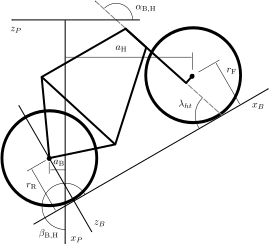
\includegraphics[width=4in]{figures/angles.pdf}
	\end{center}
	\caption{Pictorial description of the angles and dimensions that related
    the nominal bicycle reference frame $XYZ_B$ with the pendulum reference frame
    $XYZ_P$.}
	\label{fig:angles}
\end{figure}
\begin{equation}
	\beta=\lambda-\alpha
    \label{eq:frameRotAng}
\end{equation}
The pendulum axis $X_P$ is simply a line in the nominal bicycle reference frame with a slope $m$ and a z-intercept $b$. The slope can be shown to be
\begin{equation}
	m_i=-\tan{\beta_i}
\label{eq:slope}
\end{equation}
The z-intercept can be shown to be
\begin{equation}
	b_i=\frac{d_i}{\cos{\beta_i}}-r_\mathrm{R}
    \label{eq:zInt}
\end{equation}
Only two lines are required to calculate the center of mass of the laterally
symmetric frame, but more orientations increase the center of mass measurement
accuracy. The three lines are defined as:
\begin{equation}
   y = m_ix+b_i
   \label{eq:line}
\end{equation}
The CoM location can be calculated by finding the intersection of these three
lines. Two approaches were used used to calculate the center of mass. Intuition
leads me to think that the center of mass is located at the centroid of the
triangle made by the three intersecting lines. The centroid can be found by
calculating the intersection point of each pair of lines and then averaging the
three intersection points.
\begin{equation}
	\left[
	\begin{array}{cc}
		-m_1 & 1\\
		-m_2 & 1
	\end{array}
	\right]
	\left[
	\begin{array}{c}
		x_a\\
		z_a
	\end{array}
	\right]
	=
	\left[
	\begin{array}{c}
		b_1\\
		b_2
	\end{array}
	\right]
\label{eq:linearSystem}
\end{equation}
\begin{equation}
    x_\mathrm{B} = \frac{x_a + x_b + x_c}{3}
\end{equation}
\begin{equation}
    z_\mathrm{B} = \frac{z_a + z_b + z_c}{3}
\end{equation}
Alternatively the three lines can be treated as an over determined linear
system and the least squares method is used to find a unique solution. This
solution is not at the centroid of the triangle made by the intersecting lines.
I am not sure which solution is theoretically the correct one for the location
of the center of mass.
\begin{equation}
	\left[
	\begin{array}{cc}
		-m_1 & 1\\
		-m_2 & 1\\
		-m_3 & 1
	\end{array}
	\right]
	\left[
	\begin{array}{c}
        x_\mathrm{B}\\
        z_\mathrm{B}
	\end{array}
	\right]
	=
	\left[
	\begin{array}{c}
		b_1\\
		b_2\\
		b_3
	\end{array}
	\right]	
\label{eq:leastSquares}
\end{equation}
\subsection{Fork}
The center of mass of the fork is calculated in the same fashion, only the
z-intercept is different.
\begin{equation}
    b = r_\mathrm{F} + \frac{a}{\cos{\beta}} + w\tan{\beta}
\end{equation}
\section{Moment of Inertia}
The moments of inertia of the wheels, frame and fork were measured by taking
advantage of the assumed symmetry of the parts and by hanging the parts as both
compound and torsional pendulums and measuring the period of oscillation when
perturb at small angles. The rate of oscillation was measured was measured
using a \href{http://www.siliconsensing.com/CRS03}{Silicon Sensing CRS03 100
deg/s rate gyro}. The rate gyro was sampled at
1000hz with a
\href{http://sine.ni.com/nips/cds/view/p/lang/en/nid/14604}{National
Instruments USB-6008 12 bit data acquisition unit} and
Matlab. The measurement duration were either 15 or 30 secs and each moment of
inertia measurement was performed three times. No extra care was taken to
calibrate the rate gyro, maintain a constant power source (i.e. the battery
drains slowly), or account for drift. The raw voltage signal was used to
determine only the period of oscillation which is need for the moment of inertia
calculations.
\subsection{Torsional Pendulum}
A torsional pendulum was used to measure all of moments of inertia about axes
in the lateral symmetric plane of each of the wheels, fork and frame. The
pendulum is made up of a rigid mount, an upper clamp, a torsion rod, and
various lower clamps.
A 5mm diameter, 1m long mild steel rod was used as the torsion
spring. A lightweight, low relative moment of inertia clamp was constructed
that could clamp the rim and the tire. The wheel was hung freely such that the
center of mass aligned with the torsional pendulum axis and then it was
secured. The wheel was then perturbed and it oscillated about the pendulum axis.
The rate gyro was mounted on the clamp in line with the pendulum axis. The
radial moment of inertia can can calculated as such:

\subsection{Wheels}
The wheels are assumed to be symmetric laterally and about any radial axis. Thus only two
moment's of inertia are required. The moment of inertia about the axle was
measured by hanging the wheel as a compound pendulum. The wheel was hung on a
horizontal rod and perturbed to oscillate about the axis of the rod. This rate
gyro was attached to the spokes near the hub and orientated mostly along the
axle axis. The wheels tended to precess at the contact point about the vertical
axis. This adds a very low frequency component of rate along the vertical axis,
but should not affect the compound pendulum axis. A better fixture for the
wheel could prevent the precession. The pendulum arm length is the distance
from the rod/rim contact point to the mass center of the wheel. The inner
diameter of the rim was measured and divided by two to get $l$. The moment of
inertia about the axle is calculated by:
\begin{equation}
    I_{\mathrm{R}yy} = \left(\frac{\bar{T}}{2\pi}\right)^2m_\mathrm{R}gl_\mathrm{R} -
    m_\mathrm{R}l^2
\end{equation}

The radial moment of inertia was measured by hanging the wheel as a torsional
pendulum. A 5mm diameter, 1m long mild steel rod was used as the torsion
spring. A lightweight, low relative moment of inertia clamp was constructed
that could clamp the rim and the tire. The wheel was hung freely such that the
center of mass aligned with the torsional pendulum axis and then it was
secured. The wheel was then perturbed and it oscillated about the pendulum axis.
The rate gyro was mounted on the clamp in line with the pendulum axis. The
radial moment of inertia can can calculated as such:
\begin{equation}
    I_{xx} = \frac{k\bar{T}^2}{4\pi^2}
\end{equation}
\subsection{Frame}
\subsection{Fork}
\appendix
\section{Bicycle Descriptions}
\subsection{Yellow Bicycle}
The yellow is a bicycle used in the lab to demonstrate that a bicycle is stable
at certain speeds. It is an aluminum road frame of unknown make with the
majority of components removed. The wheels, drop handlebar, seat, seat post and
bottom bracket are the only parts on the bike. The fork has been reversed to
''increase`` the stability of the bicycle. The bicycle was measured with both
the fork in normal position and the fork reversed.
\begin{table}
	\begin{tabular}{ll}
		Style & Road\\
		Size & \\
		Wheels & 700c Aluminum Rims\\
		Tires & 28 x 1 3/8 x 1 5/8\\
		Sprocket & 6 speed free wheel\\
		Handlebars & Drop\\
	\end{tabular}
	\caption{}
	\label{yellowBikeSpecs}
\end{table}

\subsection{Batavus Browser}
The Batavus Browser is lower priced Dutch city bike. We measured the physical
properities of the stock Browser model and also the same bike with the
instrumentation used in our experiments.
\begin{table}
	\begin{tabular}{ll}
		Price          & � 449\\
		Wheel Size     & 28''\\
		Weight         & 18.7 kg\\
		Frame Size     & 54\\
		Frame material & High Tensile Steel\\
		Fork material  & Steel\\
		Rims           & Aluminum Airline\\
    Spokes         & Stainless steel\\
		Tires          & Trax Highway, 28'' x 1 5/8 x 1 3/8\\
		Handlebar      & Steel painted\\
		Handles        & Batavus Comfort\\
		Saddle         & Selle Royal 8274\\
		Dynamo         & Basta Trio\\
		Headlight      & Batavus Logic Light\\
		Rearlight      & Battery light\\
		Pedals         & Batavus plastic antislip\\
		Final          & Trelock RS42\\
		Theft chip     & Present\\
		Crank          & Aluminum\\
		Rack           & Steel\\
		Quick Binder   & Binder Trio\\
		Mudguards      & Steel\\
		Bell           & Kenlight\\
	\end{tabular}
	\caption{2008 Batavus Browser Specifications}
	\label{browserSpecs}
\end{table}

\subsection{2007 Bianchi Pista}
The Pista is a steel track bicycle. Specifications, taken from the Bianchi
website~\cite{Bianchi2009}, are as follows:
\begin{table}
	\begin{tabular}{ll}
		Style            & Track Bike\\
  	Size             & 57cm\\
  	Color            & Gang Green\\
  	Frame            & Bianchi DB CrMo, rear entry track dropouts\\
  	Fork             & CrMo\\
  	Retail Price     & \$579.99\\
		Headset          & VP AheadSet, 1''threadless\\
  	Handlebar        & Bianchi steel track, 26.0mm\\
		Stem             & Bianchi alloy\\
    Brakes/Levers    & Shimano Tiagra front brake/lever\\
		Crankset         & Truvativ Touro 1.1, 48T\\
		Bottom Bracket   & Truvativ Power Spline cartridge\\
		Chain            & KMC\\
		Sprocket         & 16T fixed cog \& 16T Freewheel\\
		Pedals           & Campus pedals\\
		Wheels           & Bianchi Alex Solo wheelset, 28h rims\\
    Tires            & Continental UltraSport, 700x23C\\
    Saddle           & Bianchi Velo\\
		Seatpost         & Bianchi alloy, 27.2mm\\
		Size             & 57cm\\ 
		Seat Tube        & 570mm\\
		Top Tube-actual  & 560mm\\
		Top Tube-virtual & 560mm\\
		Chainstay        & 383mm\\
		Fork Rake        & 28mm\\
		Head Tube Angle  & 74.5$^{\circ}$\\
		Seat Tube Angle  & 75.5$^{\circ}$\\
		Wheelbase        & 967mm\\
		Standover Height & 32''  
	\end{tabular}
	\caption{}
	\label{pistaSpecs}
\end{table}
\subsection{Gary Fisher Mountain Bike}
\subsection{Batavus Crescendo Deluxe}
	
The Batavus Crescendo Deluxe is a contemporary of all-round cycling in cool black and white. A great bike for a good end to touring. And that works fine with 8 gears, suspension fork and suspension seatpost.
\begin{table}
	\begin{tabular}{ll}
		Price             & from � 869\\
		Wheel Size        & 28''\\
		Weight            & 21.5 kg\\
		Frame Size        & 53\\
		Performance/speed & Shimano Nexus 8 speed with roller brakes\\
		Color             & White / black\\
		Brakes            & Shimano roller brakes (BR-IM50)\\
		Frame type        & Ladies mono tube frame Gentlemen trend\\
		Frame material    & Aluminum 7005\\
		Front Fork        & spring, Batavus\\
		Rims              & Aluminum Rodi VR19\\
		Spokes            & Stainless steel (adapted spoke pattern)\\
		Tires             & CST End\\
		Handlebar         & Steel aluminum look\\
		Stem              & Manually adjustable, Batavus Ergo Matic III\\
		Handles           & adjustable Batavus Ergo Grip II\\
		Saddle            & Selle Royal 5160\\
		Seatpost          & spring, Post Modern Compact\\
		Dynamo            & Shimano Hub Dynamo\\
		Headlight         & Trelock Hi-Power automatic halogen\\
		Rear              & Smart battery automatically\\
		Pedals            & aluminum antislip\\
		Final							& AXA Defender\\
		Chip theft        & Present\\
		Crank             & Aluminum\\
		Rack              & Aluminum\\
		Quick Binder      & Binder Quattro\\
		Mudguards         & Batavus hyalite II\\
		Bell              & Bibia Touring\\
		Balhoofdset       & VP semi-integrated, oversized\\
		Shifters          & Batavus (8-speed)\\
		Saddlebag         & Batavus saddlebag with plakset\\
	\end{tabular}
	\caption{}
	\label{crescendoSpecs}
\end{table}
\subsection{Batavus Stratos Deluxe}
\begin{table}
	\begin{tabular}{ll}
		Switching           & Spin System (shifter)\\
		Monochromatic frame & Black\\
		Chain guard         & Semi-open\\
		Mudguards           & Aluminum\\
		Rack                & Yes\\
		Extra drive         & Regardless Motori degree\\
		Type                & Men's\\
		Frame Material      & Aluminum\\
		Rim Material        & Aluminum\\
		Rear braking system & Roller brake\\
		Front braking system & Roller Brake\\
		Number of gears      & 7 Gears\\
		Gear System          & Shimano Nexus\\
		Wheel Size           & 28 inch\\
		Tirewidth            & 37 mm\\
		Price                & 749,00\\
	\end{tabular}
	\caption{}
	\label{stratosSpecs}
\end{table}
\bibliographystyle{plain}
\bibliography{bicycle}
\end{document}
